\subsection{part a}
In condition without controller from architector $C(s) = 1$ and $F(s) = 0$.
\begin{itemize}
	\item all figures from siso toolbox
	\begin{figure}[H]
		\caption{All figures from siso toolbox}
		\centering
		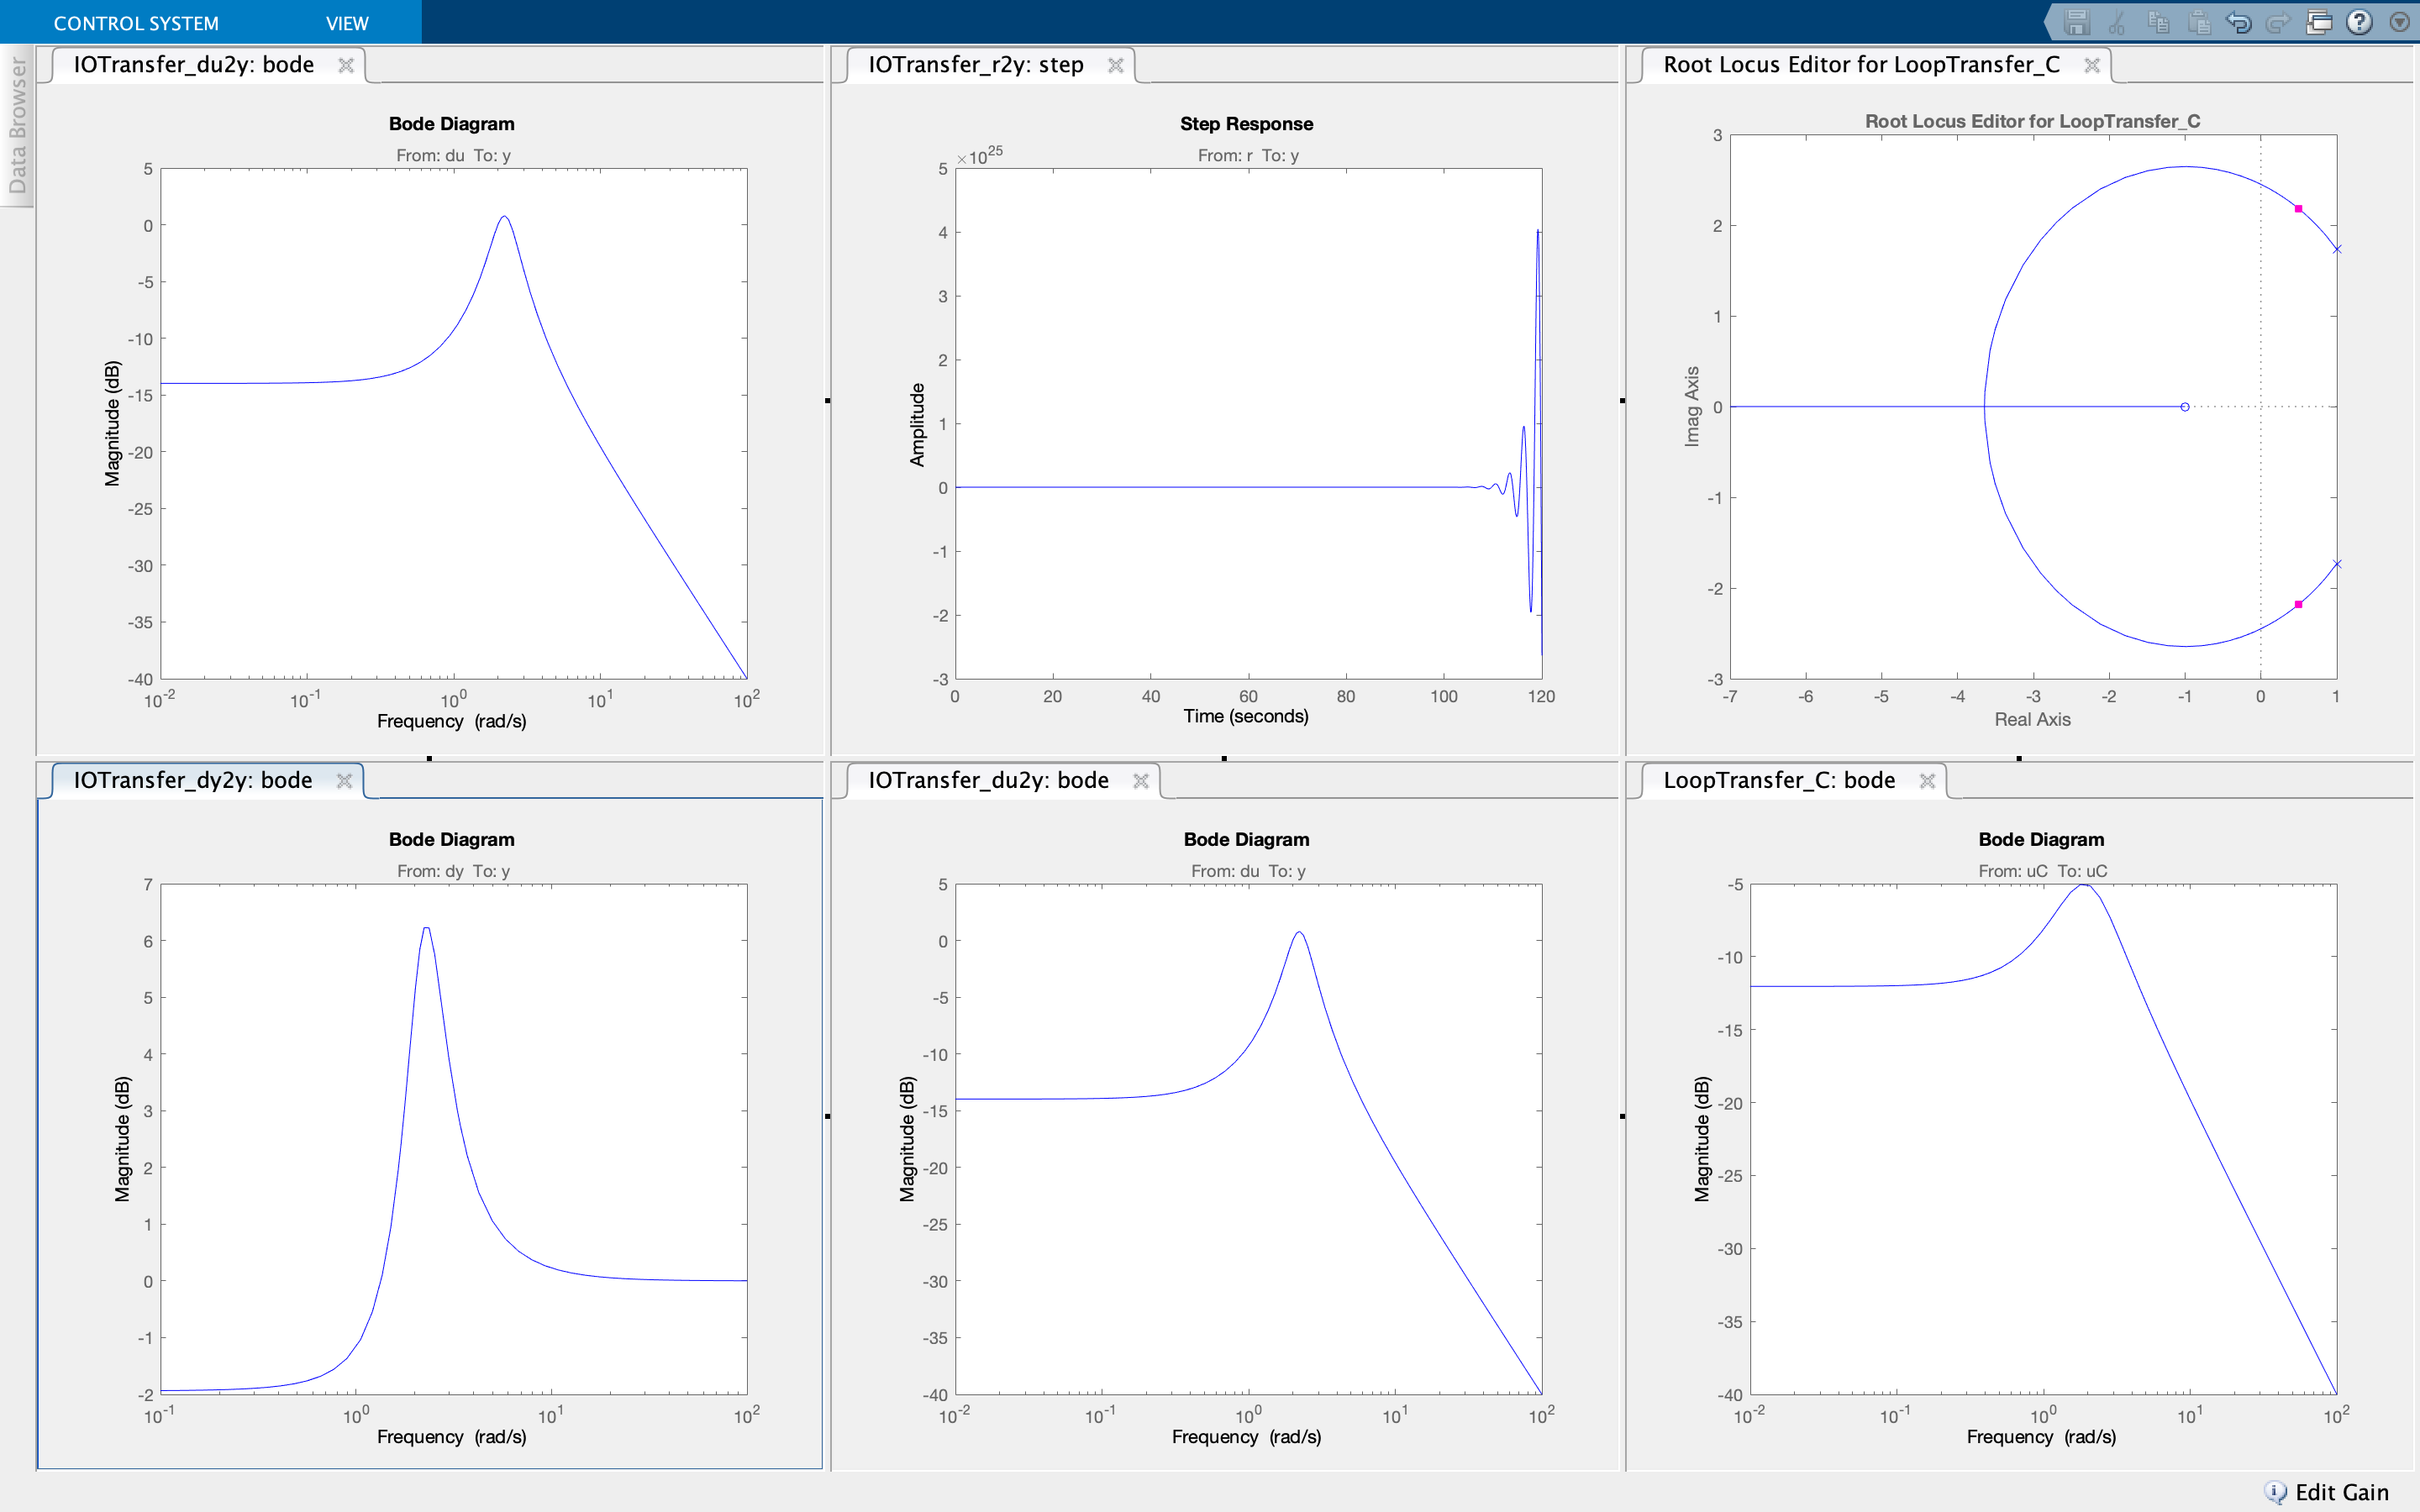
\includegraphics[width=16cm]{../Figure/Q1/Q1_a/siso_all.png}
	\end{figure}
	\newpage
	\item root locus
	\begin{figure}[H]
		\caption{root locus}
		\centering
		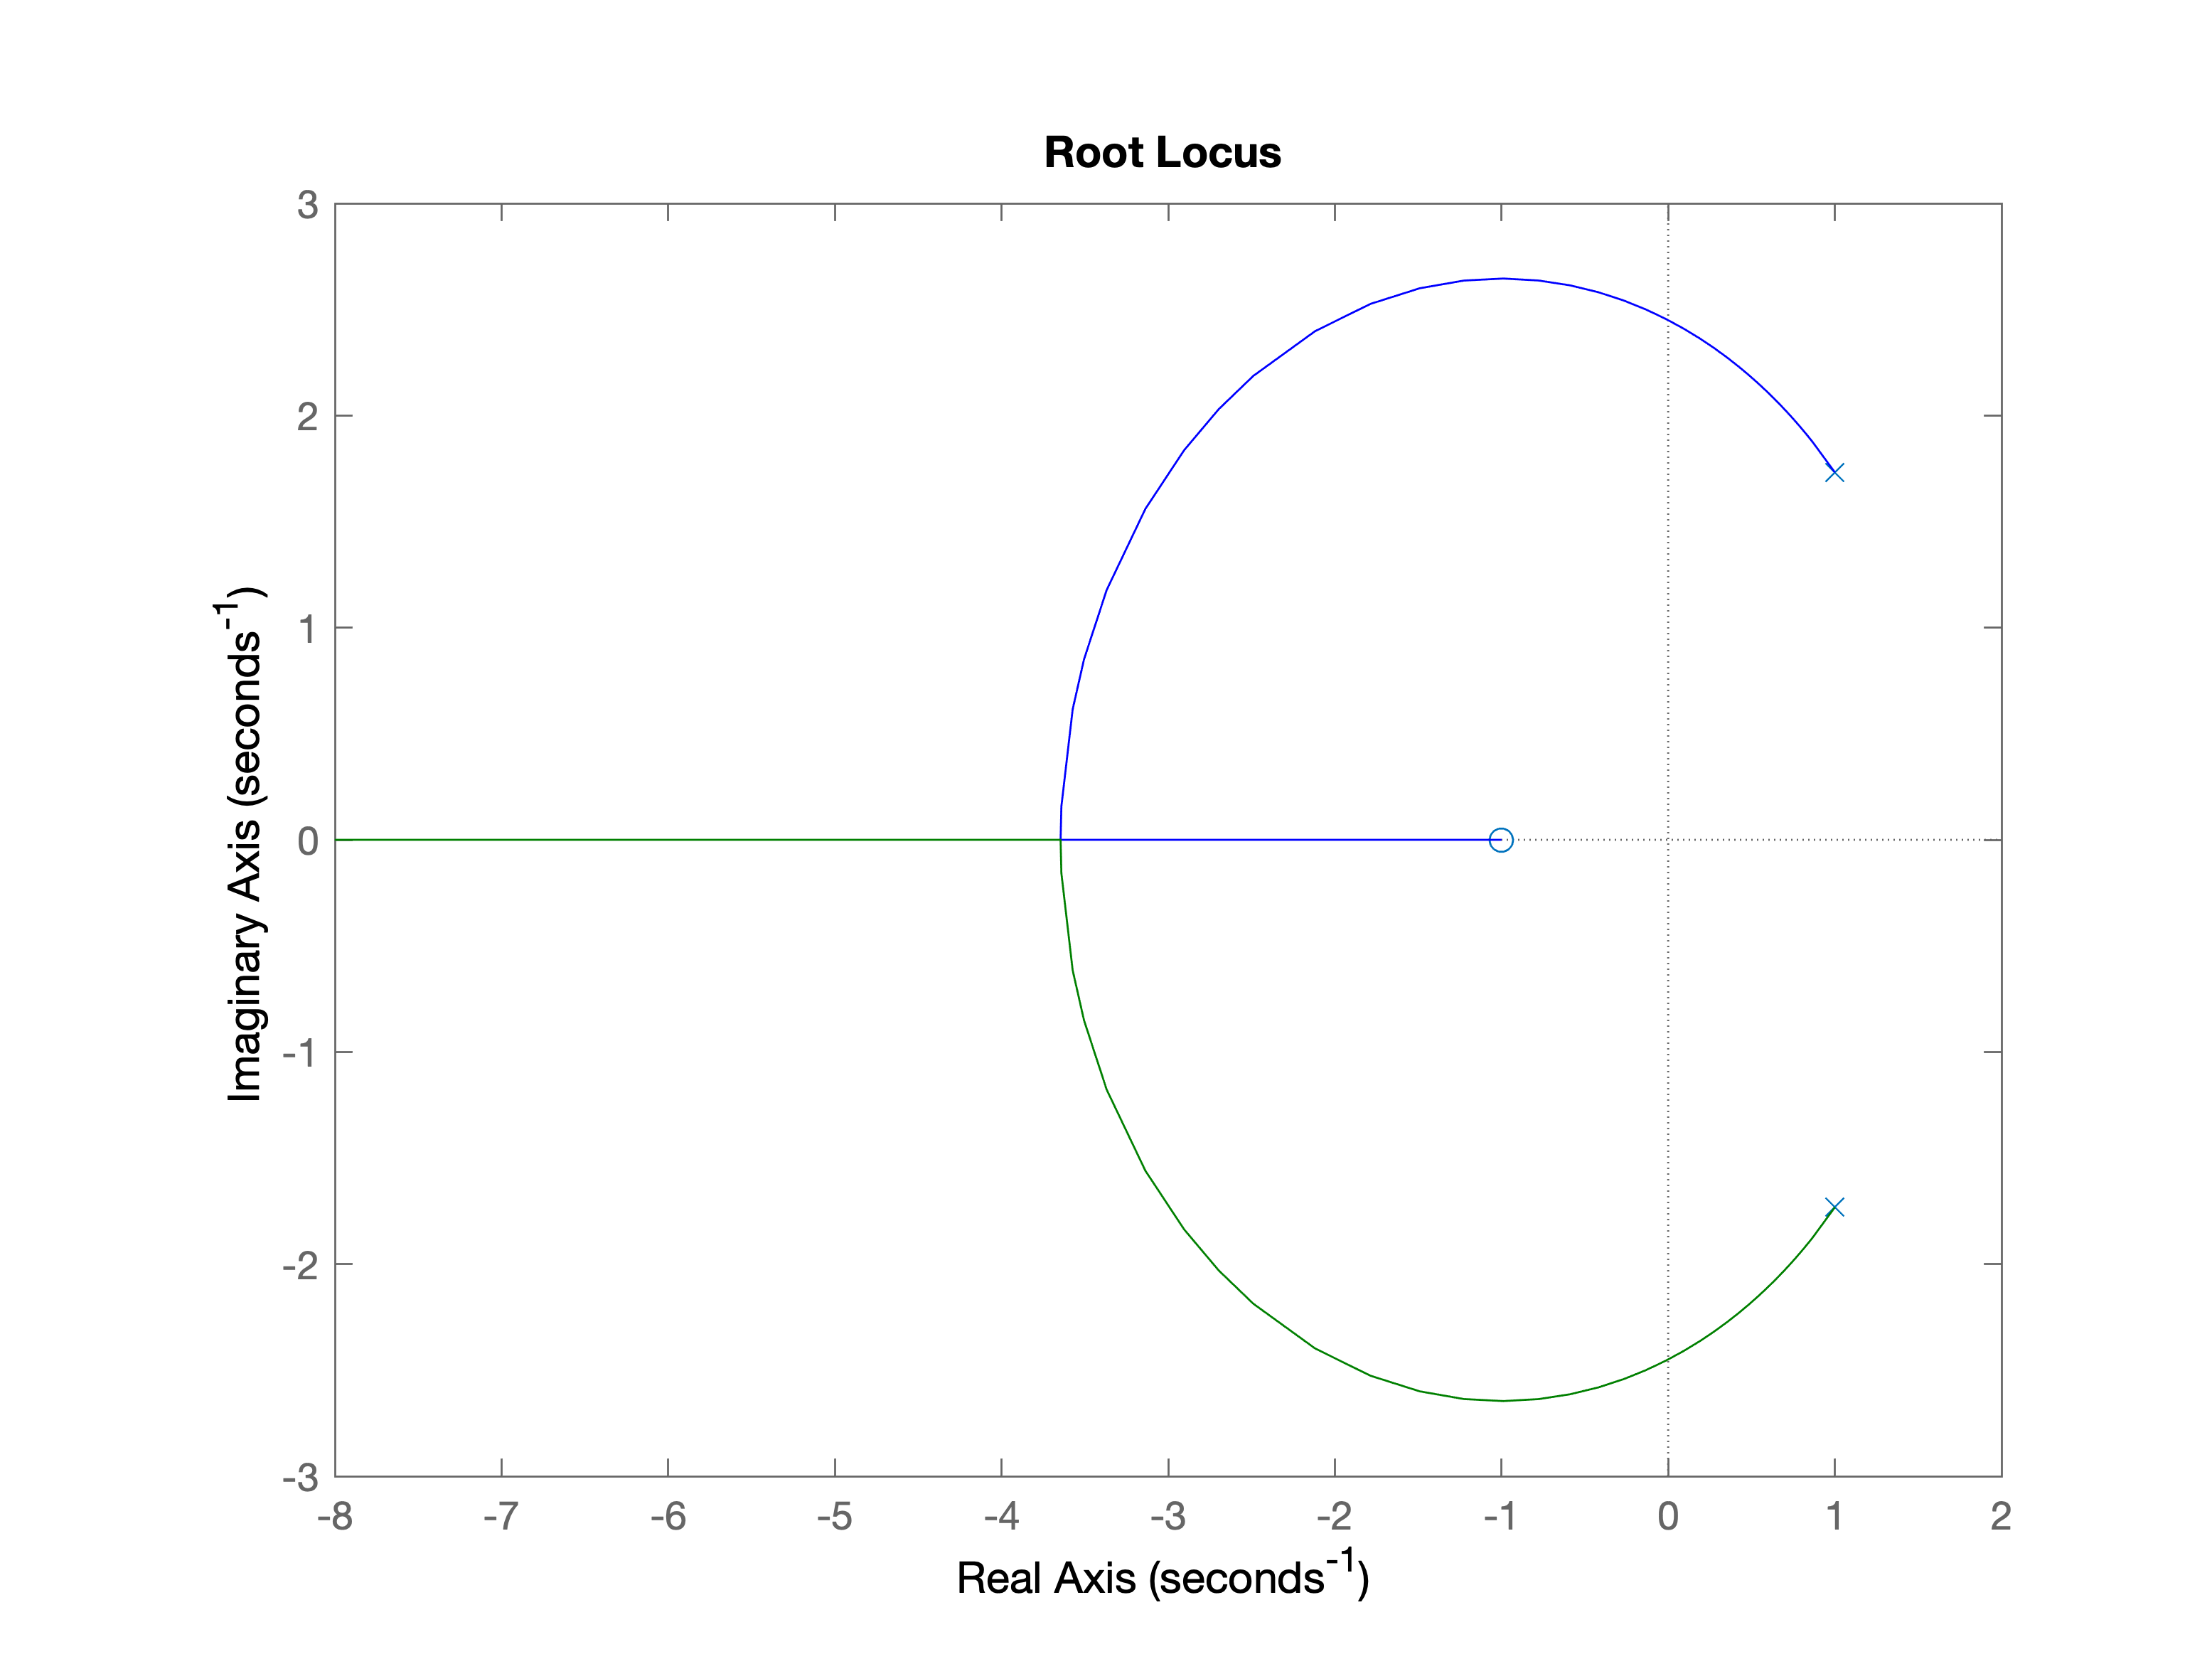
\includegraphics[width=12cm]{../Figure/Q1/Q1_a/rlocus.png}
	\end{figure}
	\item step response for closeloop system
	\begin{figure}[H]
		\caption{step response for closeloop system}
		\centering
		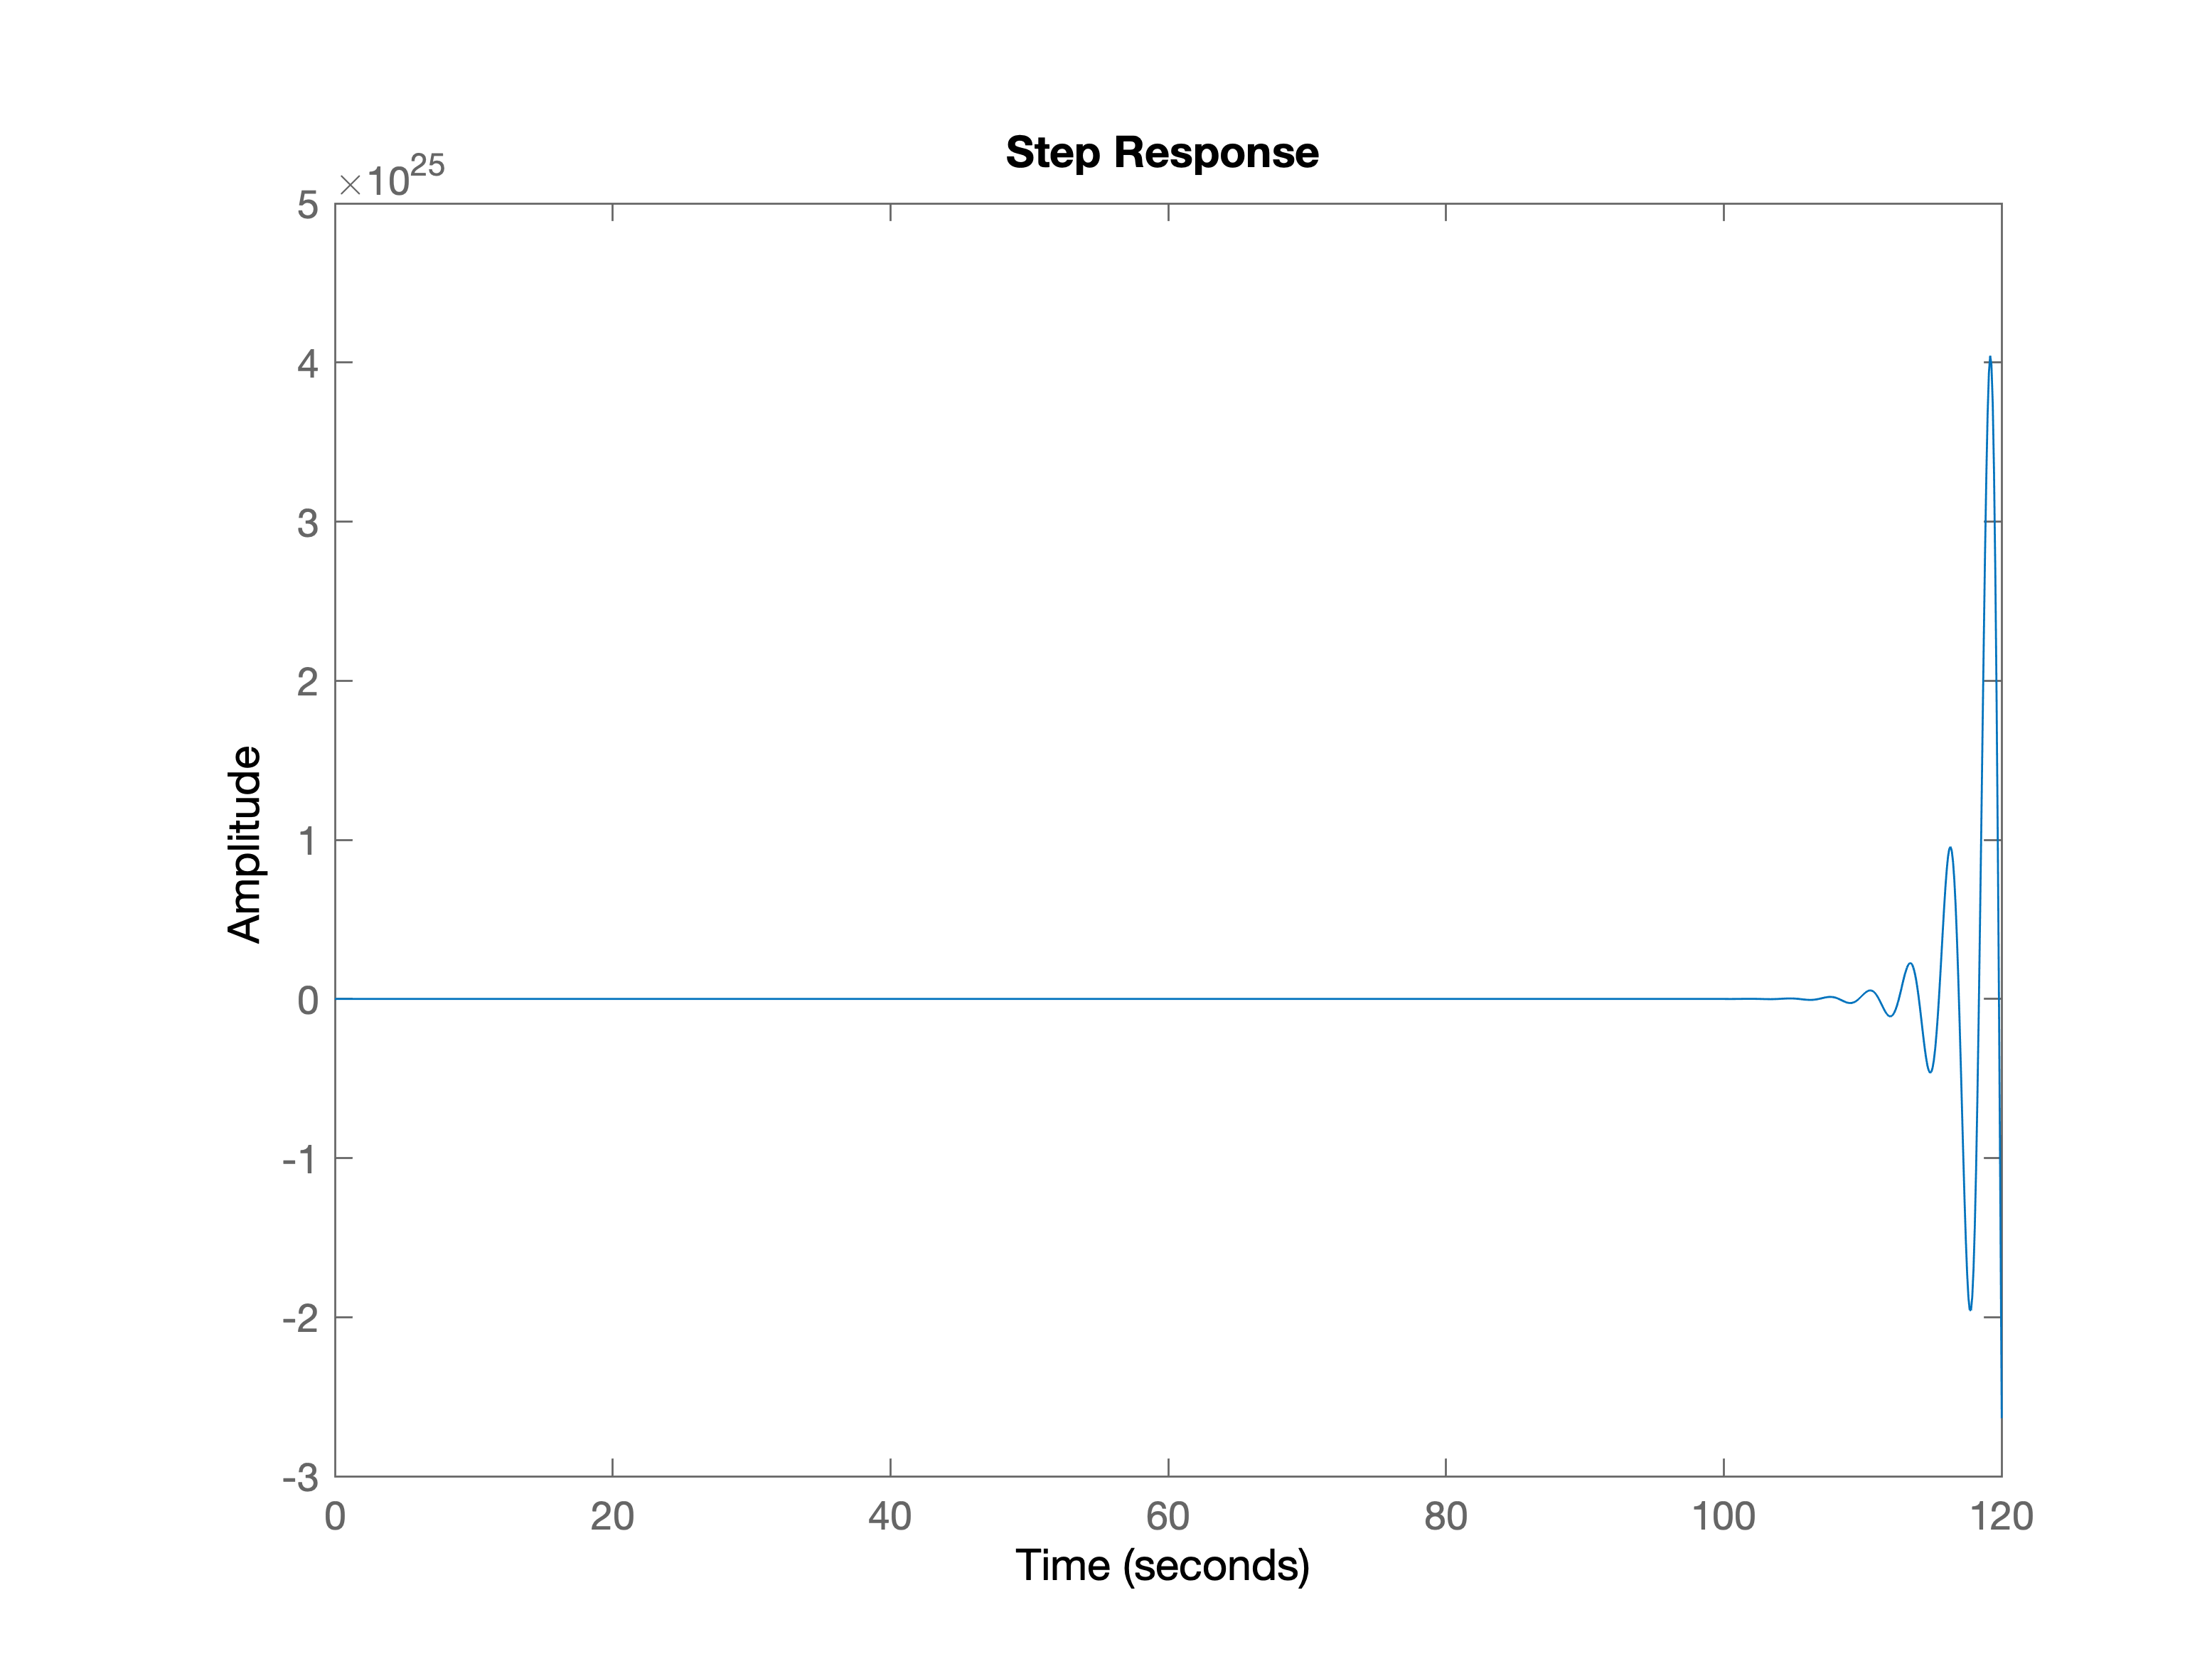
\includegraphics[width=12cm]{../Figure/Q1/Q1_a/feedback_step.png}
	\end{figure}
	\item closeloop bode (magnitude)
	\begin{figure}[H]
		\caption{closeloop bode (magnitude)}
		\centering
		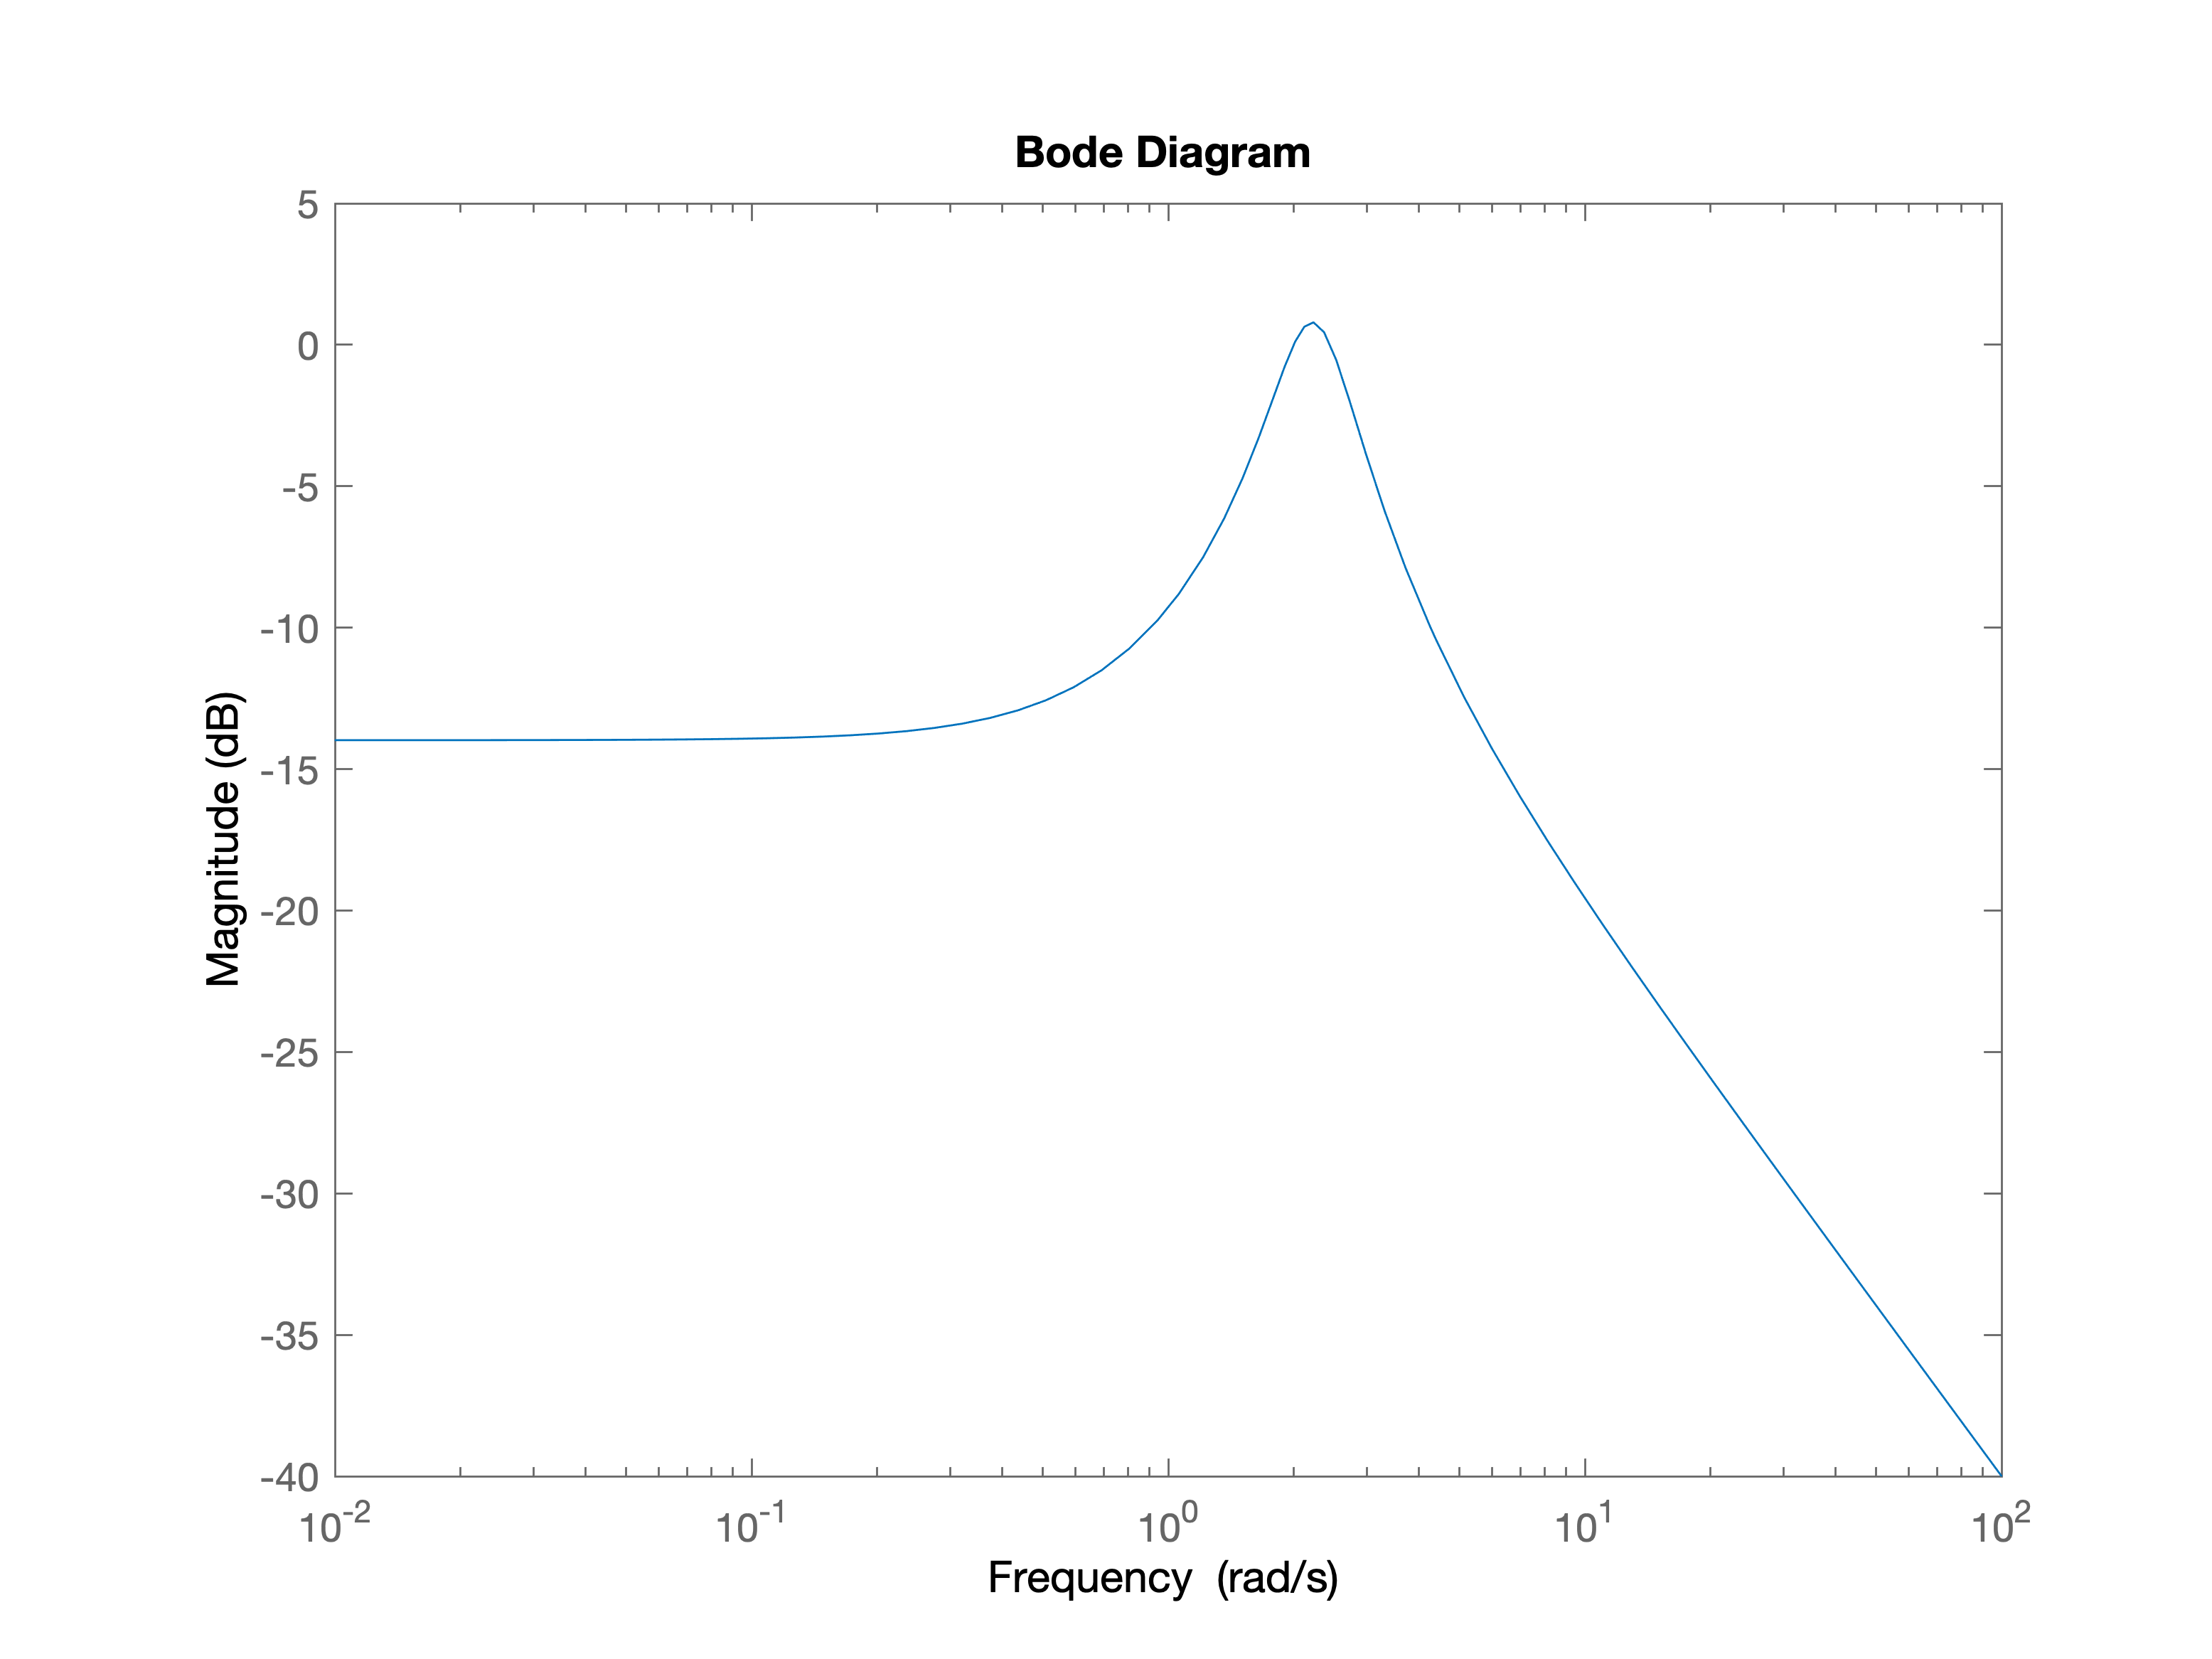
\includegraphics[width=12cm]{../Figure/Q1/Q1_a/feedback_bode.png}
	\end{figure}
	\item openloop bode (magnitude)
	\begin{figure}[H]
		\caption{openloop bode (magnitude)}
		\centering
		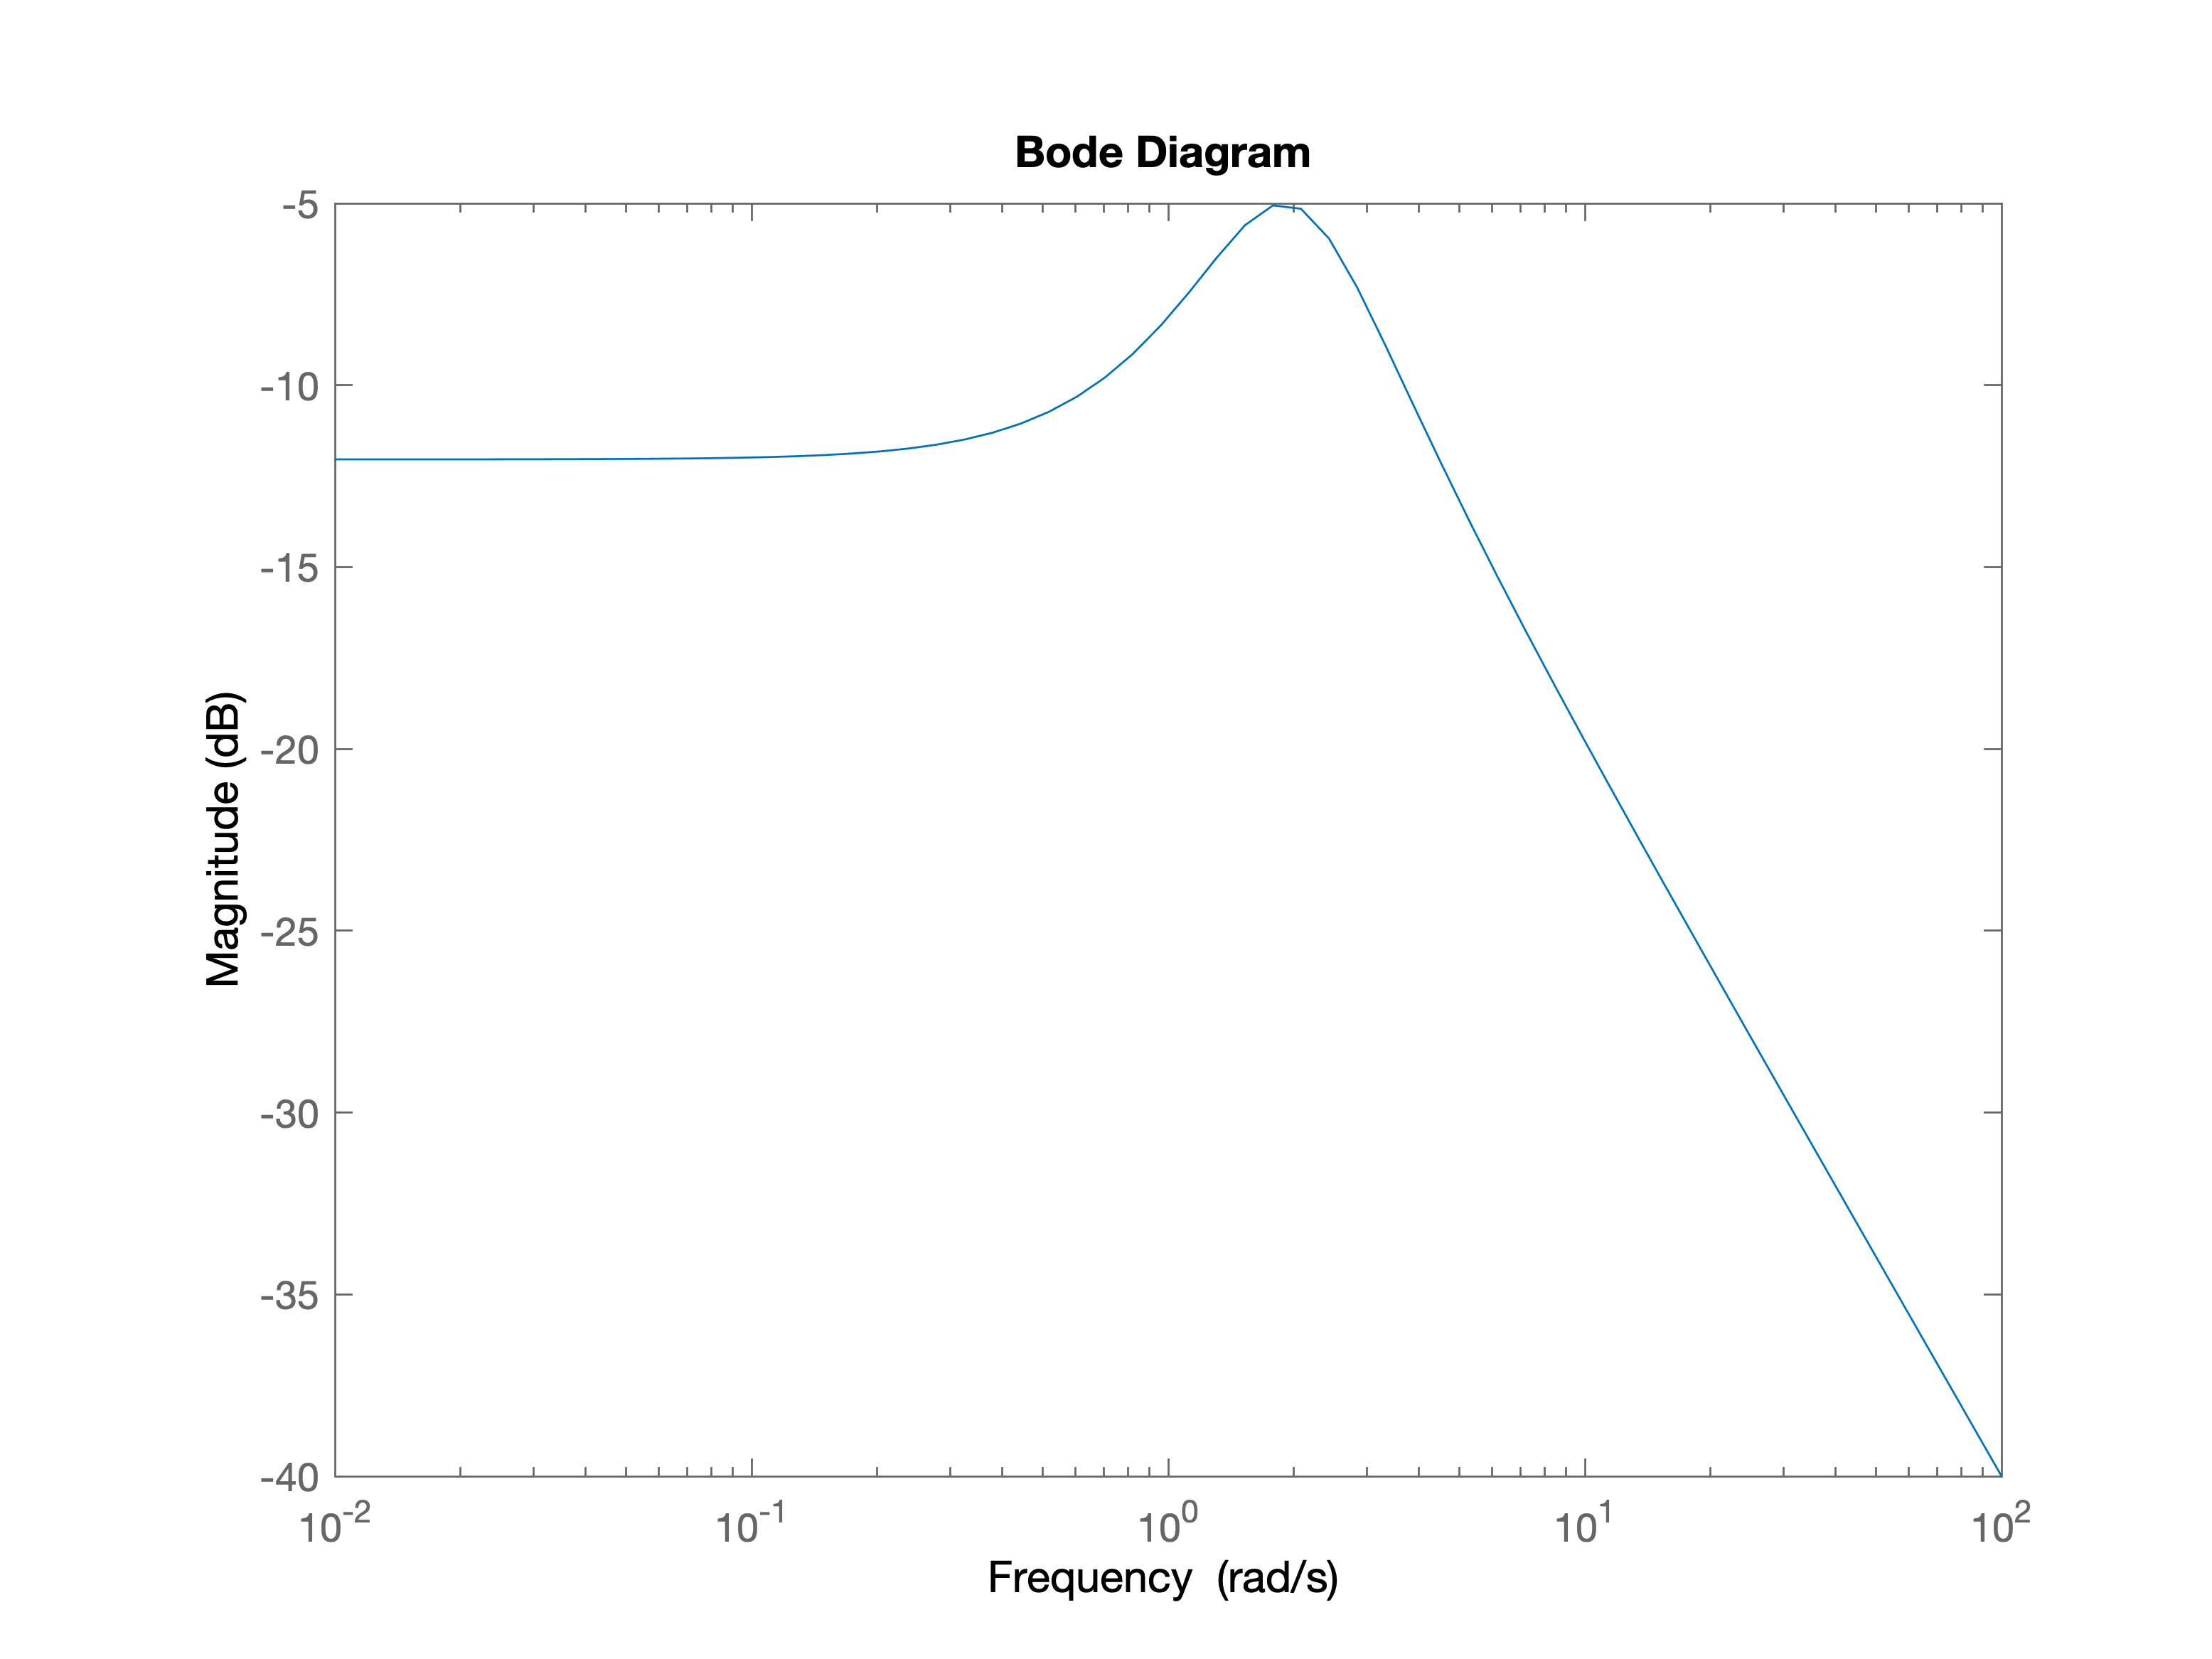
\includegraphics[width=12cm]{../Figure/Q1/Q1_a/openloop_bode.png}
	\end{figure}
	\item sensitivity function
	\begin{figure}[H]
		\caption{sensitivity function}
		\centering
		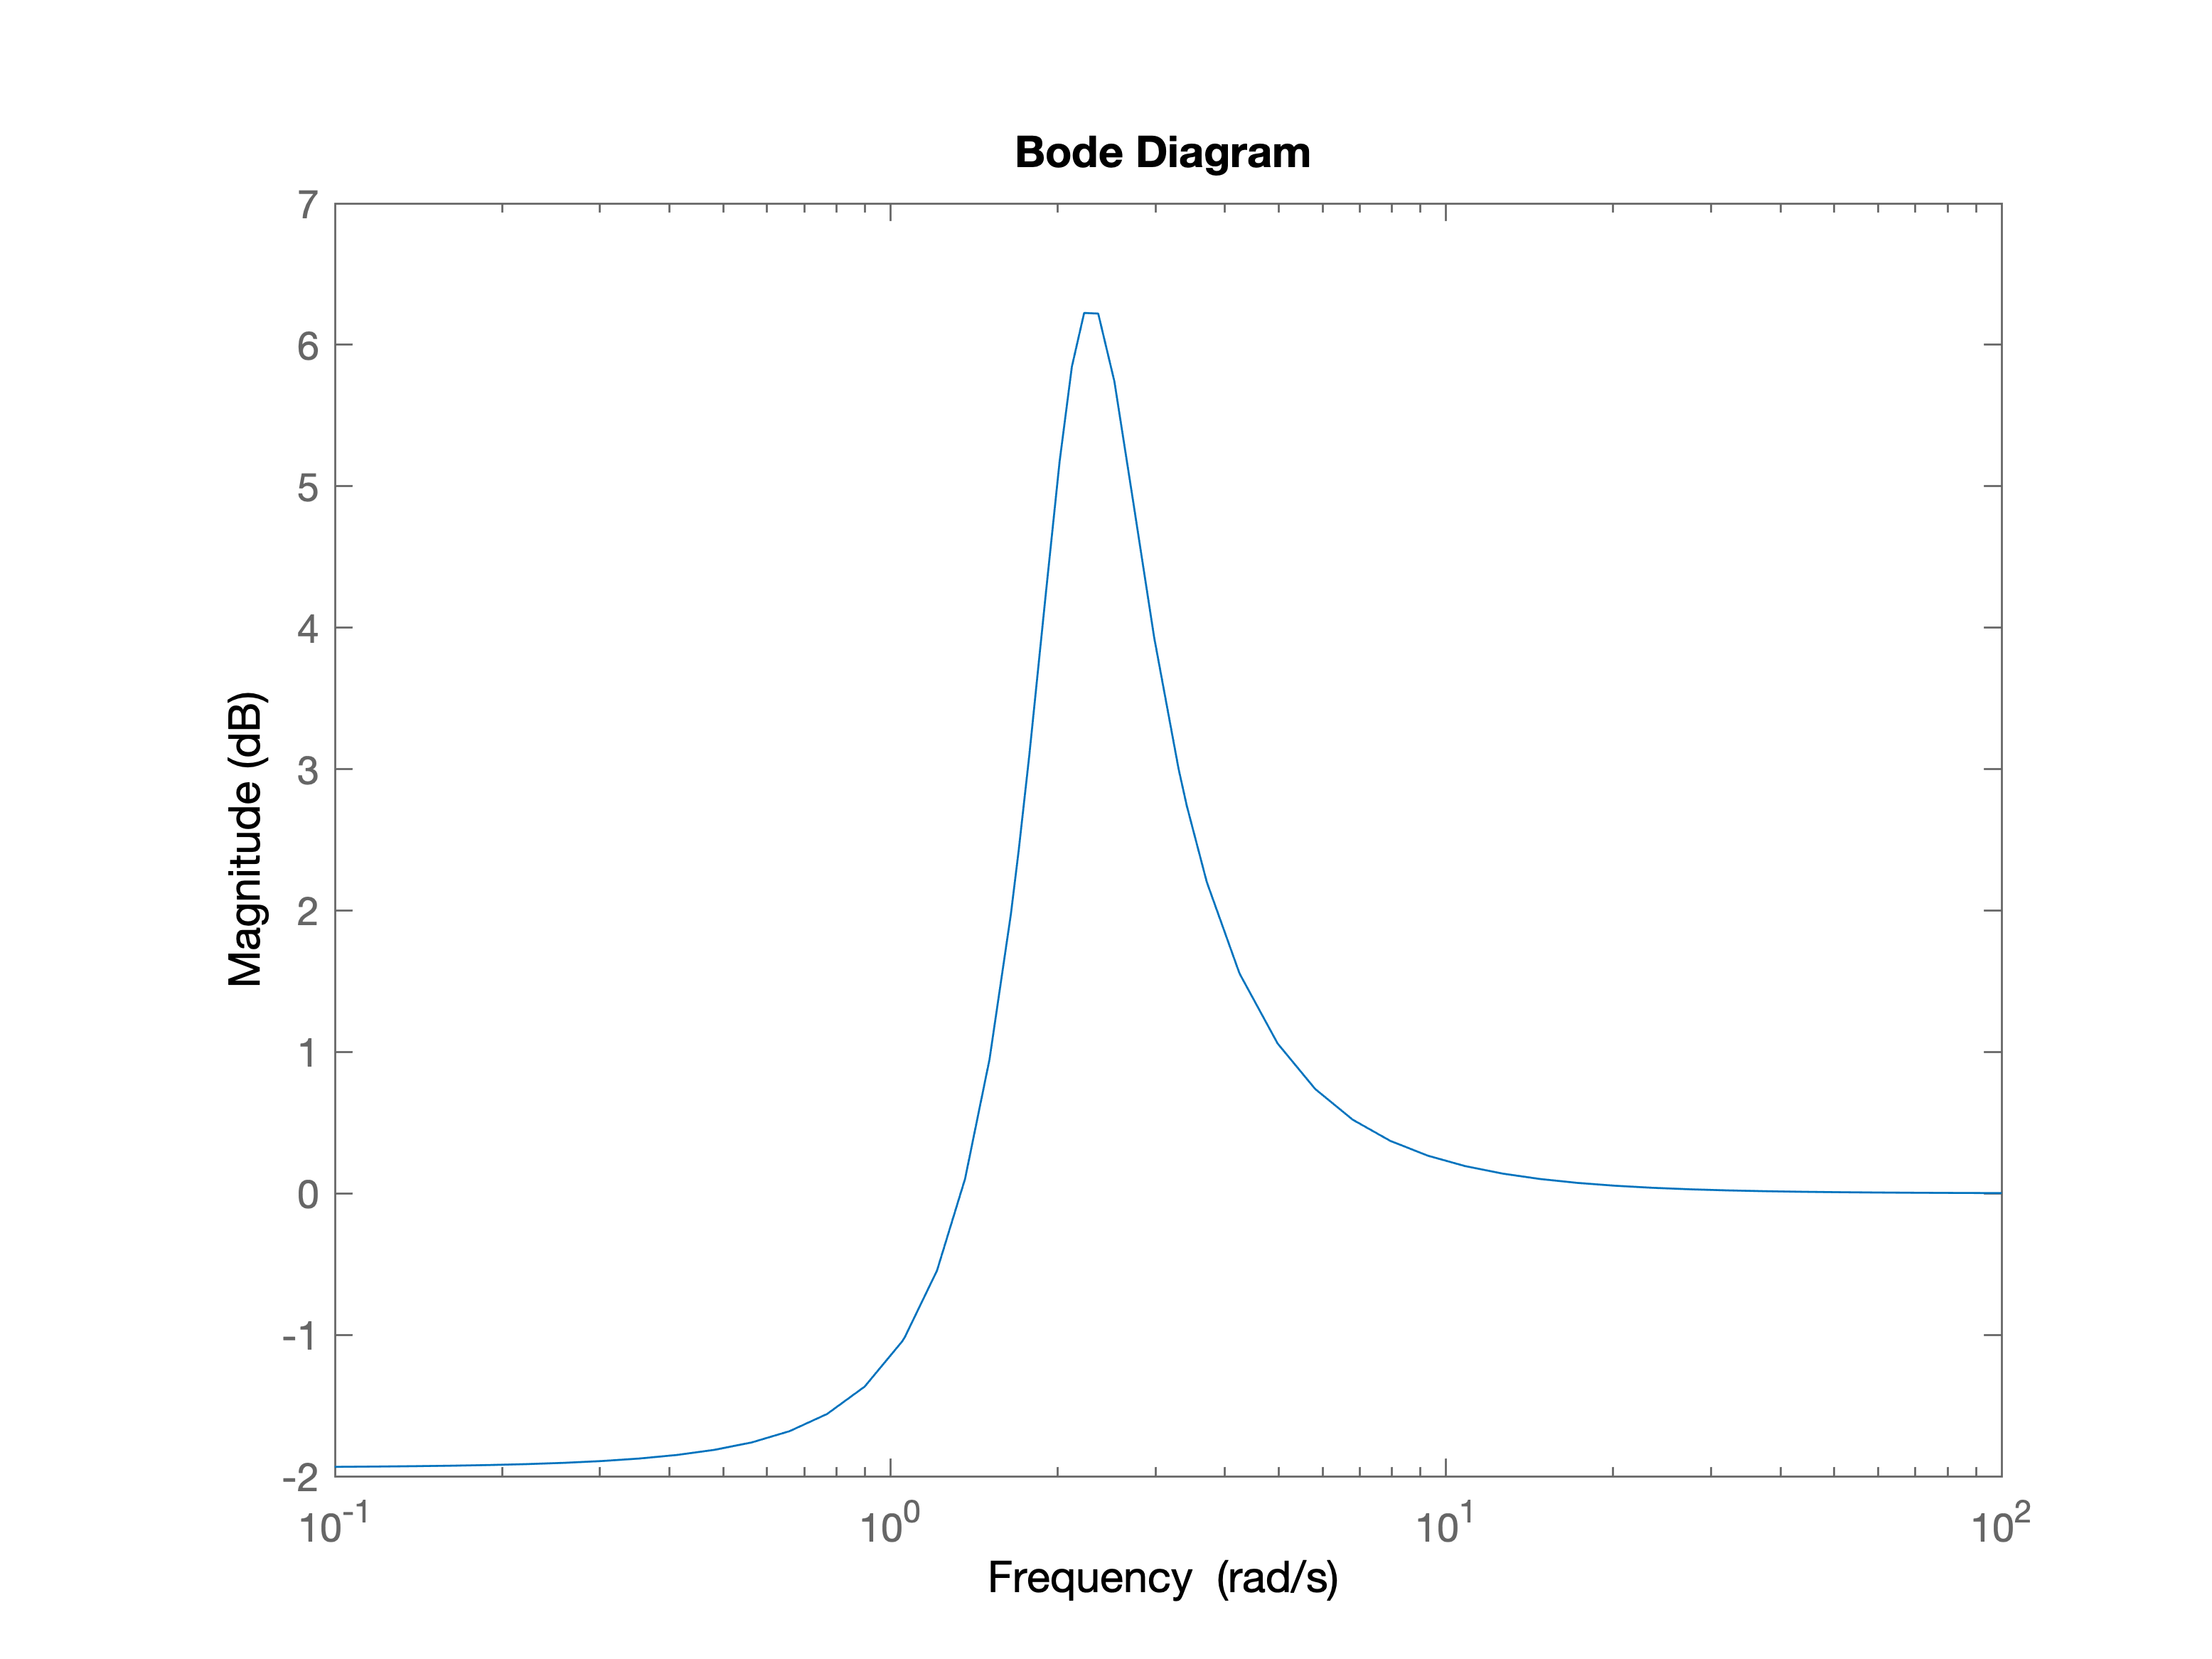
\includegraphics[width=12cm]{../Figure/Q1/Q1_a/s_bode.png}
	\end{figure}
	\item complementary sensitivity function
	\begin{figure}[H]
		\caption{scomplementary sensitivity function}
		\centering
		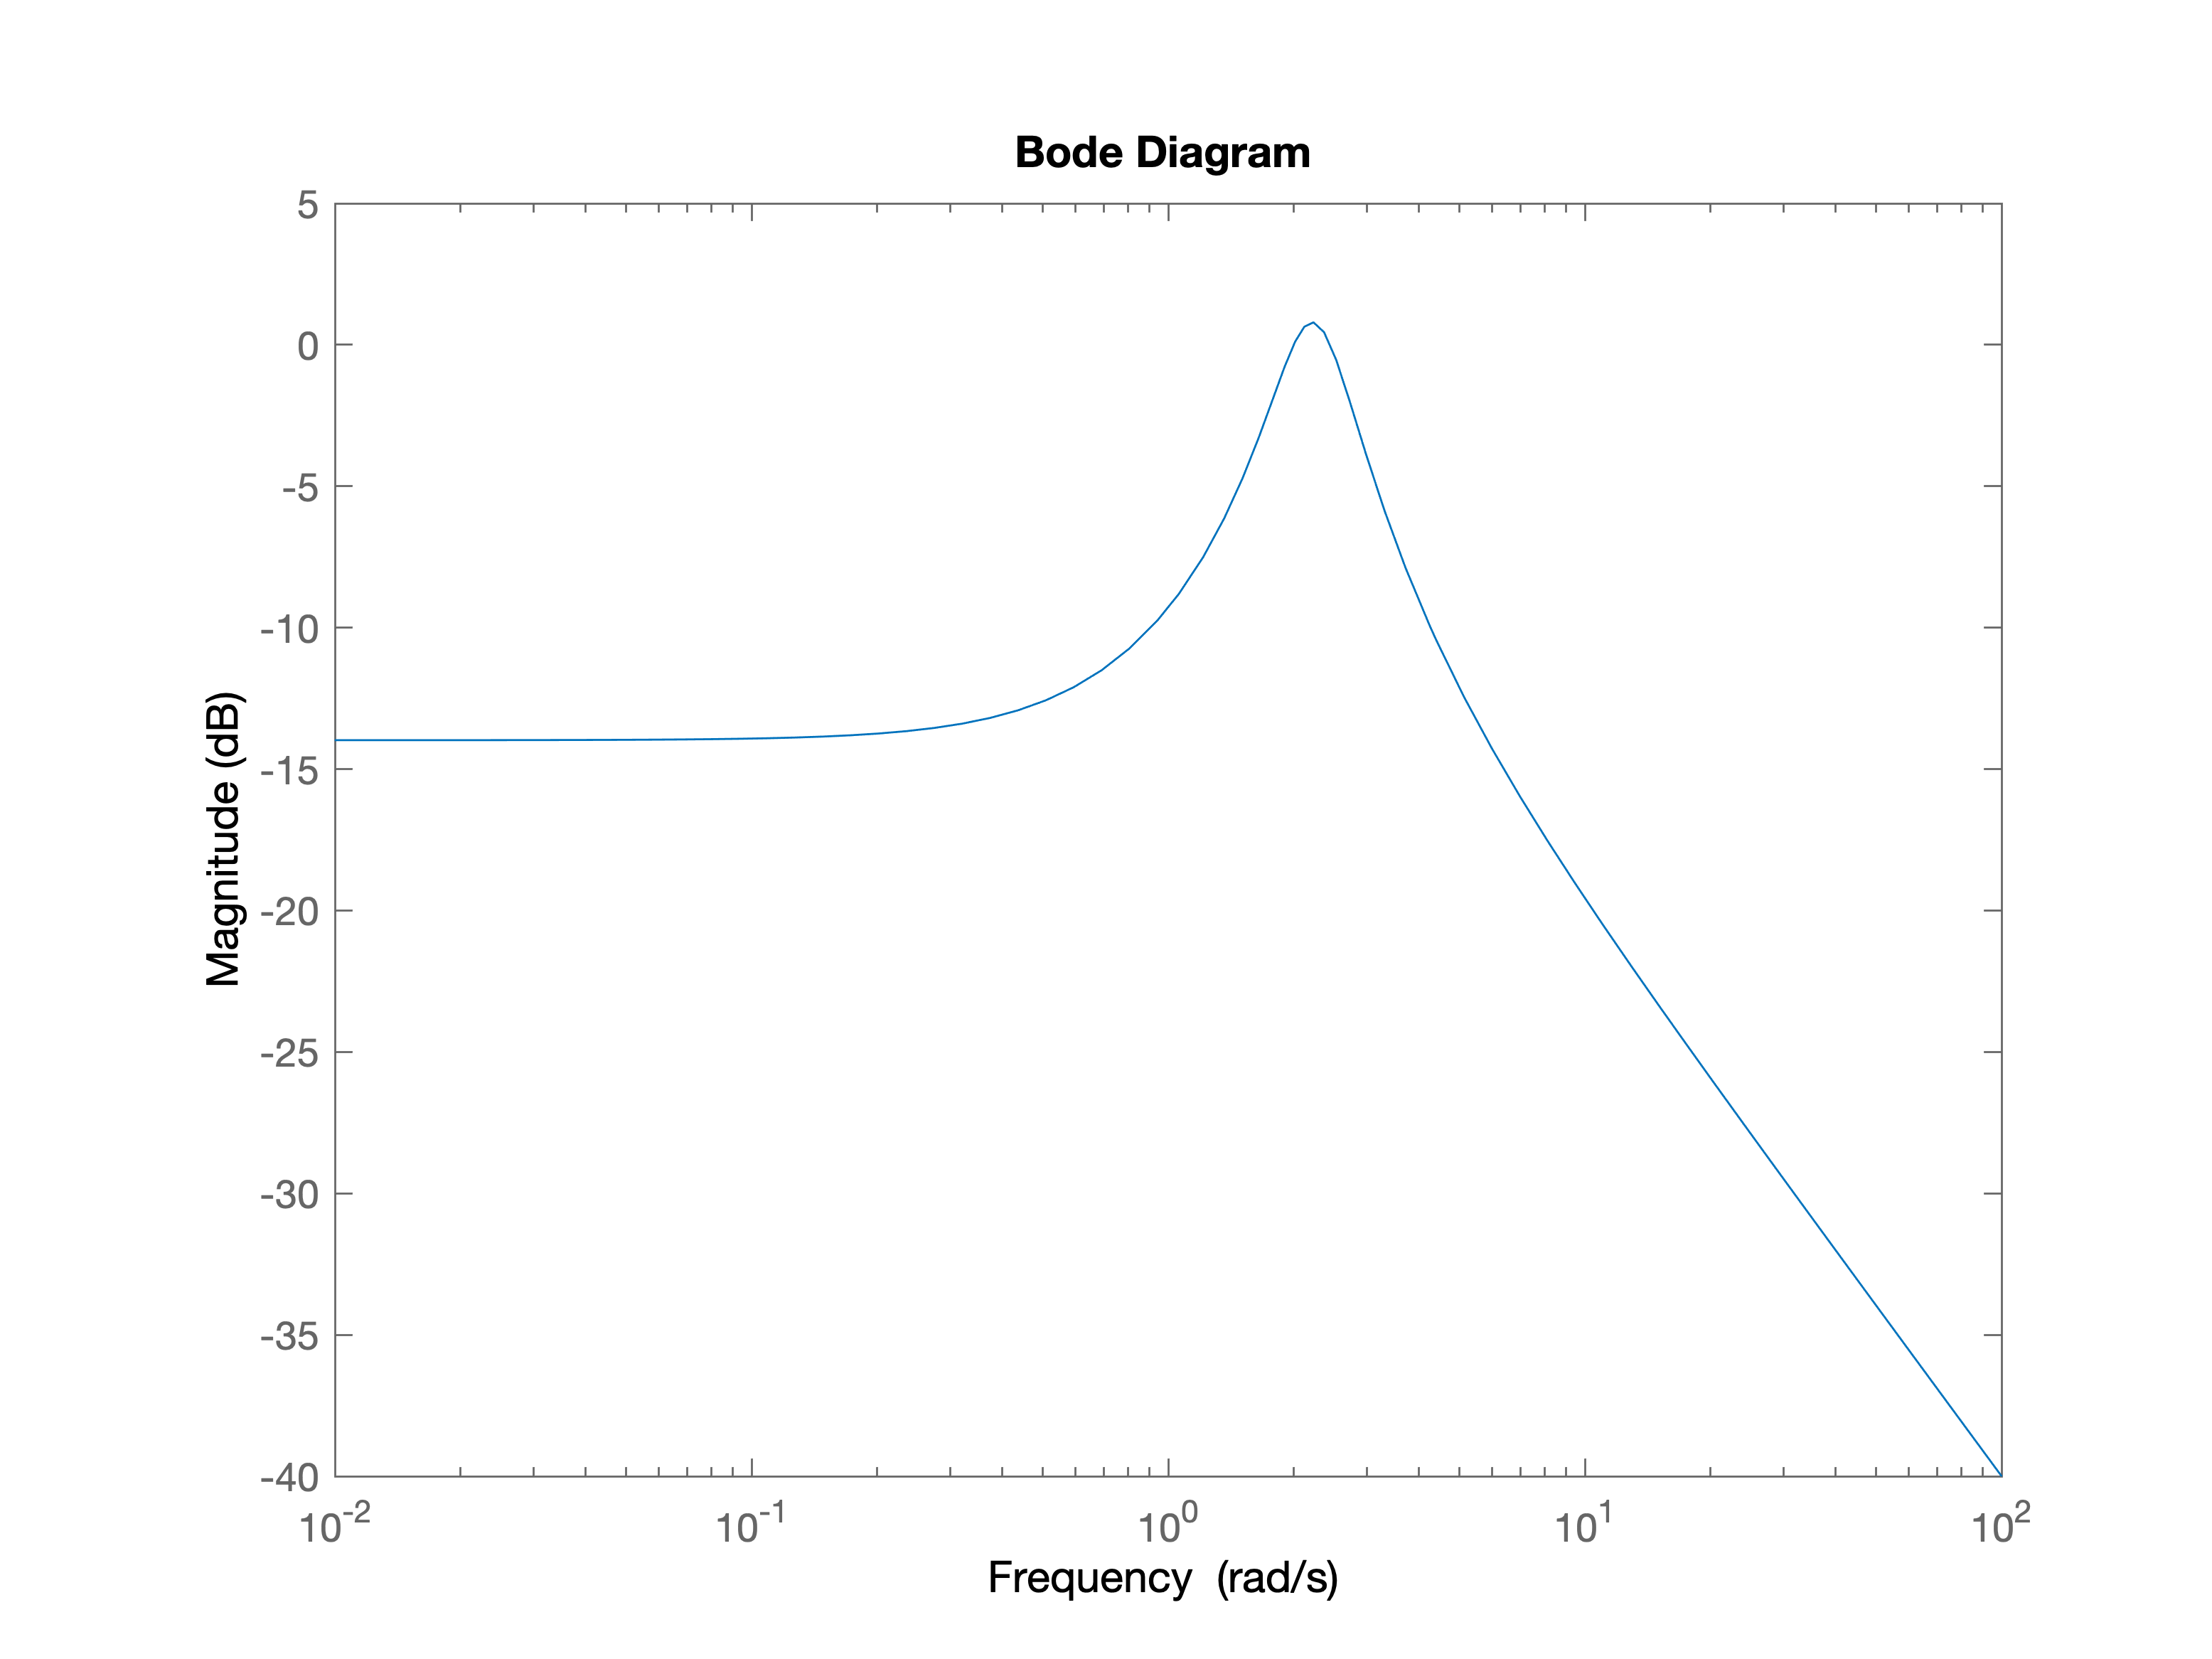
\includegraphics[width=12cm]{../Figure/Q1/Q1_a/t_bode.png}
	\end{figure}
\end{itemize}